\section{Framework Overview}
% problem definition and data analysis[SDM13]
In this section, the proposed framework \textit{KSTR} is presented. As can be seen in Figure~\ref{fig:framework}, \textit{KSTR} is comprised of two modules: the offline pattern discovery and scoring module and the online travel routes exploration module. % The description for each module is as follows:
\vspace{-3mm}

\begin{figure}[h]
\centering
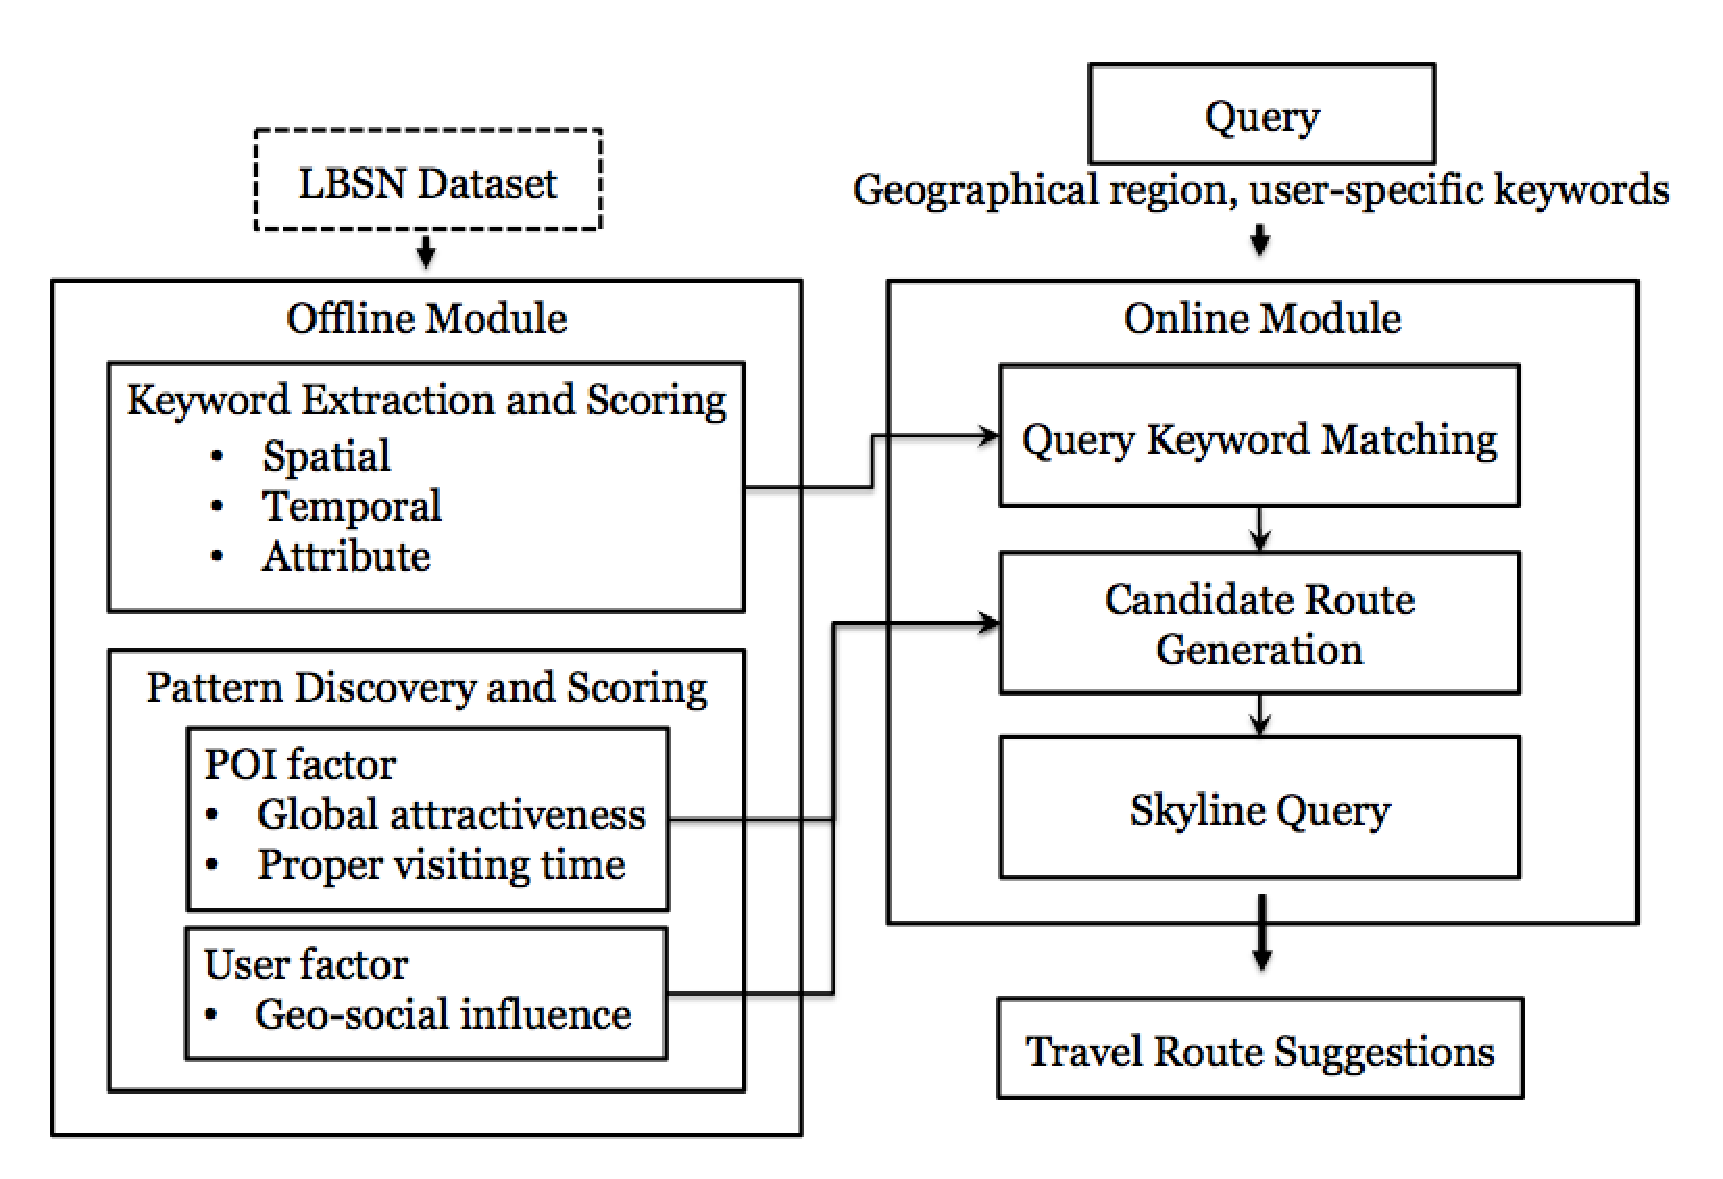
\includegraphics[width=\linewidth]{framework.eps}
\caption{The overview of the proposed \textit{Keyword-aware Skyline Travel Route} framework}
\label{fig:framework}
\end{figure} 

\textbf{Offline pattern discovery and scoring module:} Given an LBSN dataset, we first analyze the tags of each POI to determine the semantic meaning of the keywords, which are classified into (i) Geo-specific keywords, (ii) Temporal keywords and (iii) Attribute keywords according to their features. Then, we define the attractiveness scores and the proper visiting time of the POIs. For this goal, we translate the trajectories into a region transition graph, in which the vertices represent POIs and edges indicate the transition relationships among POIs. Furthermore, we determine the proper visiting time of each POI by analyzing the population distribution with timestamps, and assigning a time score for each time interval. Besides the global features that produce the same results for different people, social influence considers the geo-social networks for each user. In short, the main task of the offline module is to decide a set of POIs and derive their scores for each feature.

\textbf{Online travel routes exploration module:} In this module, we provide an interface for users to specify query ranges and preference-related keywords. With the map interface provided, users could simply input their query range as a rectangle, decide the time period to stay, and add keywords for personalized preference. Once it receives a specified range and time, the online module will retrieve those trajectories that overlap the query range and reconstruct proper travel routes in the stay time period. Then, the online module will compute a matched score of how well the trajectory is connected to the keywords. Consequently, the online module returns the most representative trajectories considering the aforementioned three scores to the users in our trajectory search Web interface. % The detailed design for the online module will be described later.